\documentclass{article}
\usepackage[T1]{fontenc}
\usepackage[utf8]{inputenc}
\usepackage{indentfirst}
\usepackage{float}
\usepackage{natbib}
\usepackage{graphicx}
\usepackage{grffile}
\usepackage{epsfig}
\usepackage{soul}
\usepackage{pdflscape}
\usepackage{hyperref}
\usepackage[scaled]{helvet}
\renewcommand\familydefault{\sfdefault} 
\usepackage[T1]{fontenc}
\usepackage[a4paper, total={16cm, 25cm}]{geometry}

\title{\textbf{Database's Models}}
\date{March 23, 2020}

\author{\textbf{Nutr.io}}

\begin{document}

\maketitle

\section{Conceptual Model}

\begin{figure}[H]
    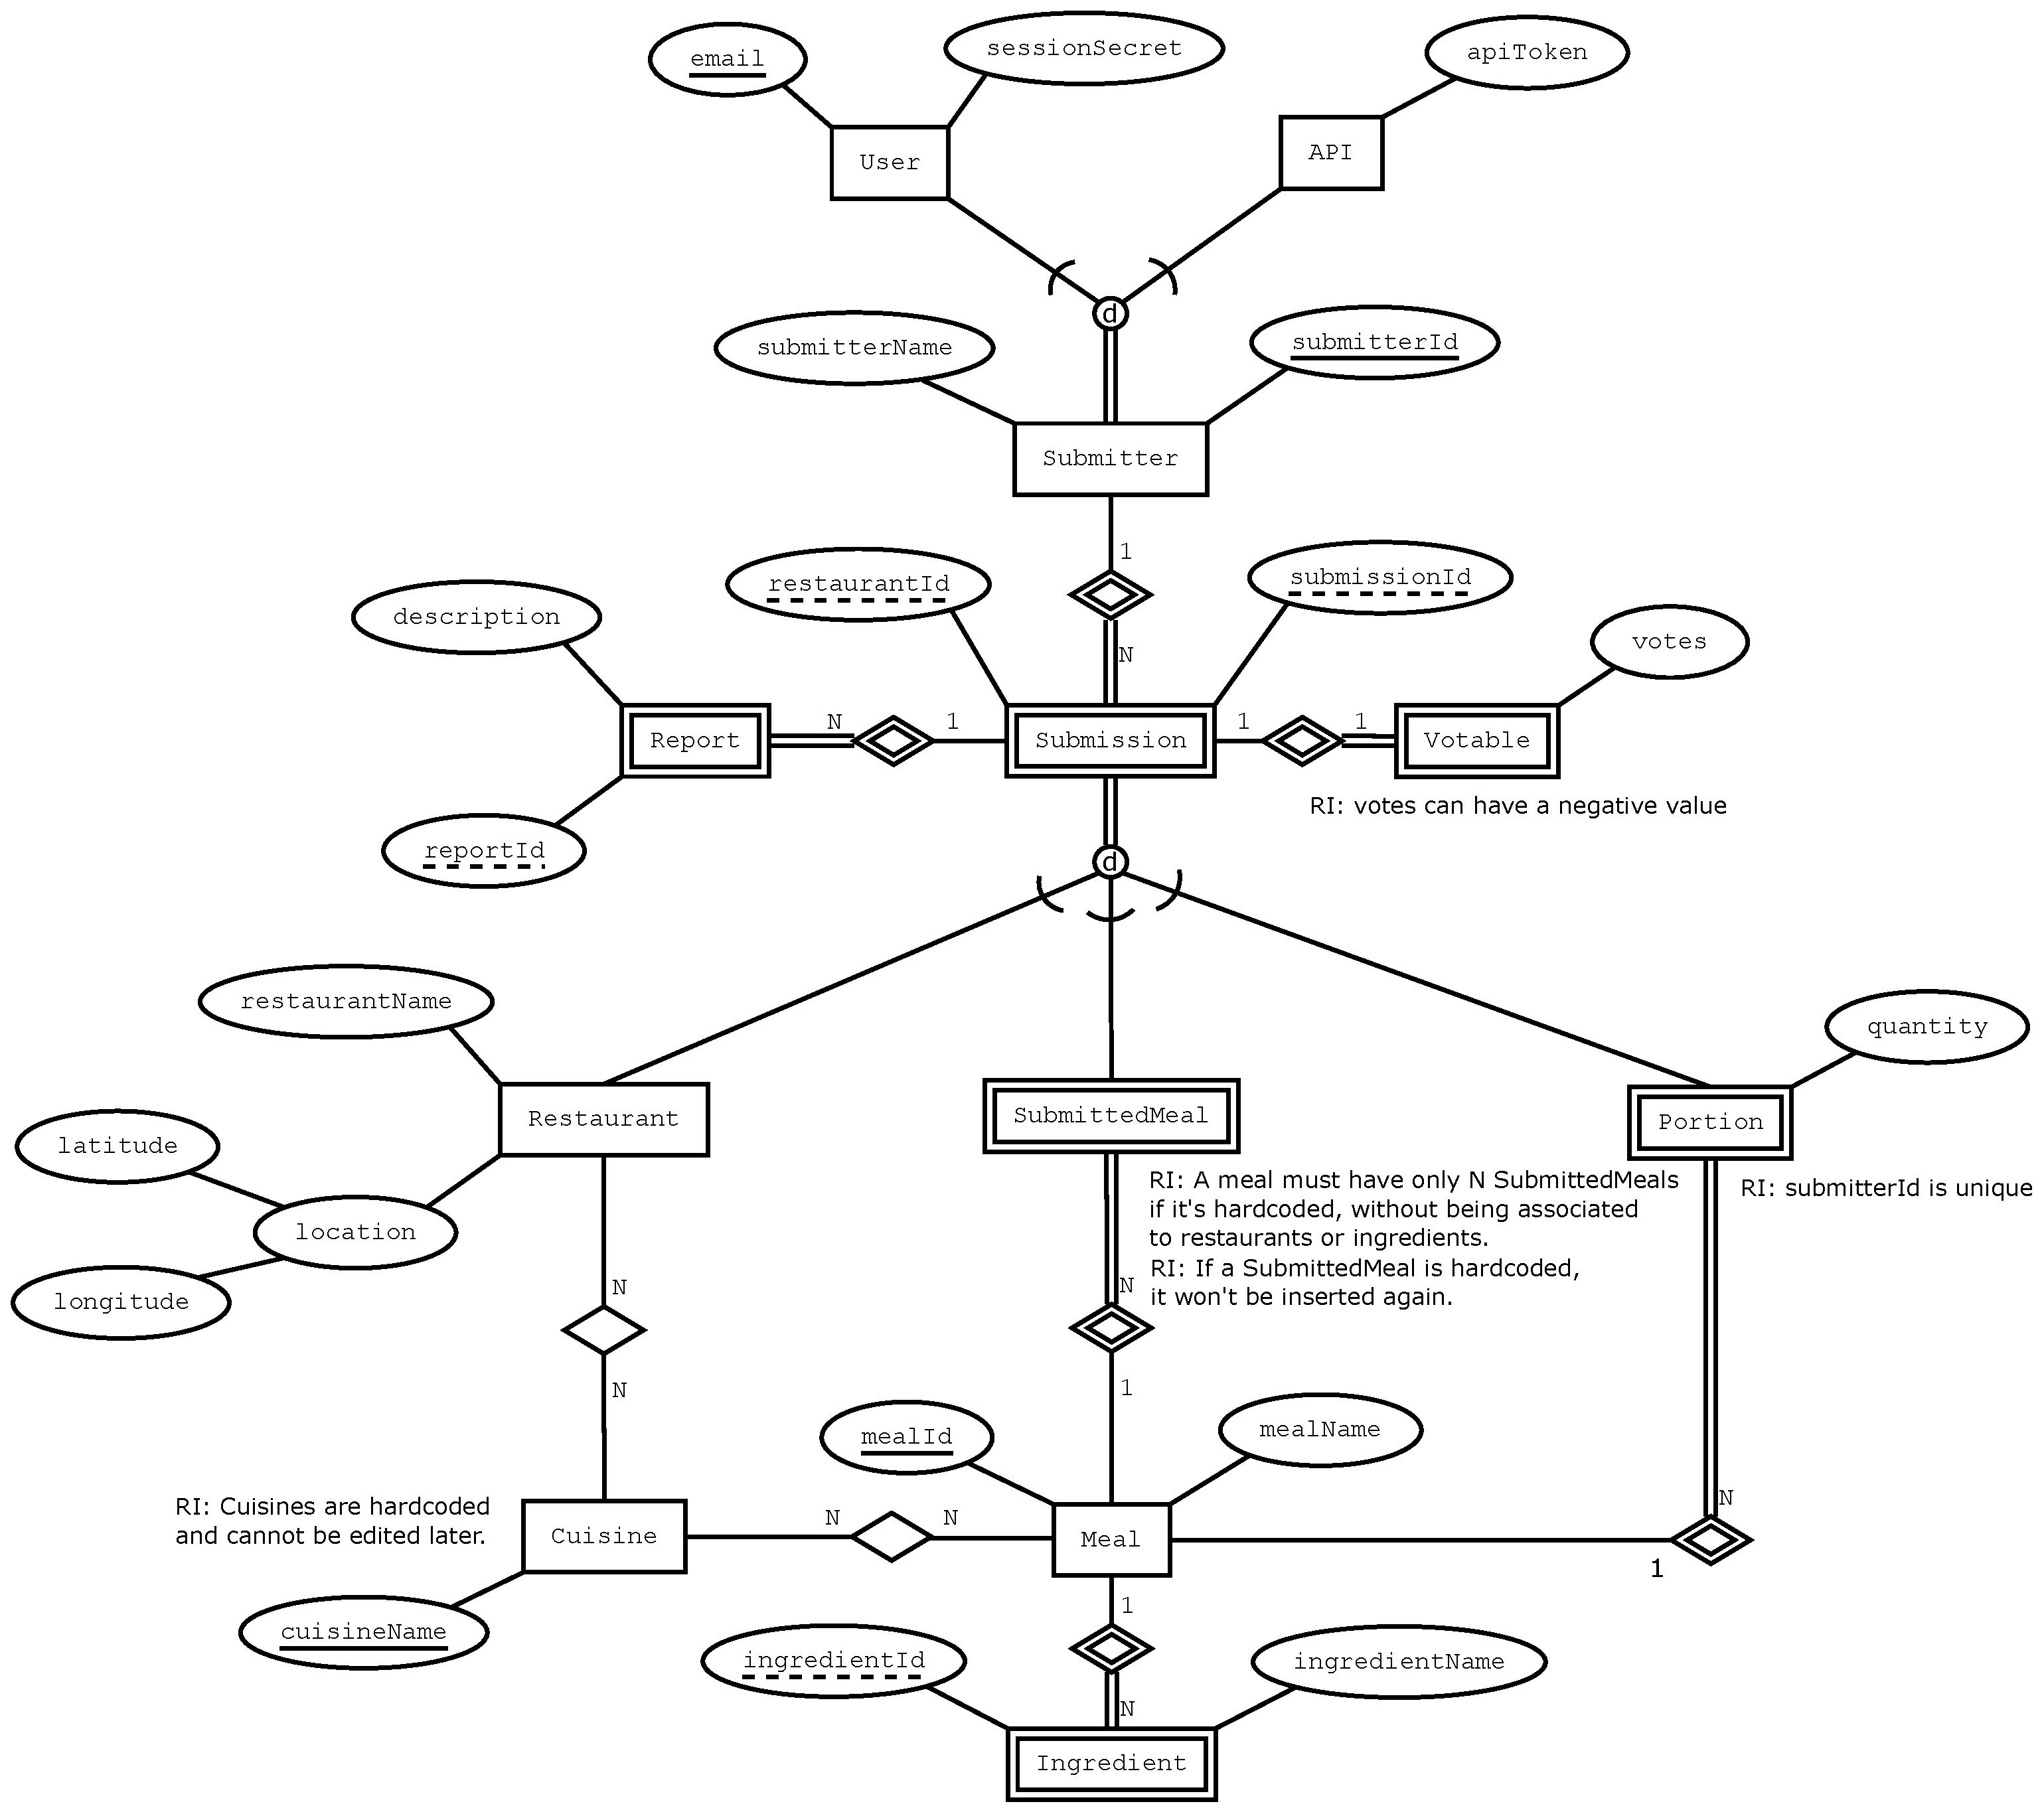
\includegraphics[scale=0.33]{Nutr.io_Database_Diagram.eps}
    \centering 
\end{figure}
\newpage

\section{Relational Model}
    \begin{itemize}
        \item \textbf{Submitter}        
        \begin{itemize}
            \item Attributes: \underline{submitterId}, submitterName, submitterType
            \item Primary Key(s): \underline{submitterId}
            \item Foreign Key(s): -
        \end{itemize}

        \item \textbf{User}
        \begin{itemize}
            \item Attributes: \underline{email}, \underline{\textit{submitterId}}, sessionSecret, submitterName
            \item Primary Key(s): \underline{email}, \underline{\textit{submitterId}}
            \item Foreign Key(s): \underline{\textit{submitterId}} from Submitter
            \item Not null: \underline{\textit{submitterId}}
        \end{itemize}

        \item \textbf{API}
        \begin{itemize}
            \item Attributes: \underline{\textit{submitterId}}, apiToken, submitterName
            \item Primary Key(s): \underline{\textit{submitterId}}
            \item Foreign Key(s): \underline{\textit{submitterId}} from Submitter
        \end{itemize}

        \item \textbf{Submission}                
        \begin{itemize}
            \item Attributes: \underline{submissionId}, \underline{restaurantId}, \underline{\textit{submitterId}}, submitterType
            \item Primary Key(s): \underline{submissionId}, \underline{restaurantId}, \underline{\textit{submitterId}}
            \item Foreign Key(s): \underline{\textit{submitterId}} from Submitter
            \item Not null: \underline{\textit{submitterId}}
        \end{itemize}

        \item \textbf{Report}
        \begin{itemize}
            \item Attributes: \underline{reportId}, \underline{\textit{submitterId}}, \underline{\textit{submissionId}}, \underline{\textit{restaurantId}}, description
            \item Primary Key(s): \underline{reportId}, \underline{\textit{submitterId}}, \underline{\textit{submissionId}}, \underline{\textit{restaurantId}}
            \item Foreign Key(s): \underline{\textit{submitterId}}, \underline{\textit{submissionId}}, \underline{\textit{restaurantId}} from Submission
            \item Not null: \underline{submissionId}, \underline{restaurantId}, \underline{\textit{submitterId}}
        \end{itemize}
            
        \item \textbf{Votable}
        \begin{itemize}
            \item Attributes: \underline{\textit{submitterId}}, \underline{\textit{submissionId}}, \underline{\textit{restaurantId}}, votes
            \item Primary Key(s): \underline{\textit{submitterId}}, \underline{\textit{submissionId}}, \underline{\textit{restaurantId}}
            \item Foreign Key(s): \underline{\textit{submitterId}}, \underline{\textit{submissionId}}, \underline{\textit{restaurantId}} from Submission
            \item Not null: \underline{submissionId}, \underline{restaurantId}, \underline{\textit{submitterId}}
        \end{itemize}

        \item \textbf{Restaurant}
        \begin{itemize}
            \item Attributes: \underline{\textit{submissionId}}, \underline{\textit{restaurantId}}, \underline{\textit{submitterId}}, restaurantName, location
            \item Primary Key(s): \underline{\textit{submissionId}}, \underline{\textit{restaurantId}}, \underline{\textit{submitterId}}
            \item Foreign Key(s): \underline{\textit{submissionId}}, \underline{\textit{restaurantId}}, \underline{\textit{submitterId}} from Submission
        \end{itemize}

        \item \textbf{SubmittedMeal}
        \begin{itemize}
            \item Attributes: \underline{\textit{submissionId}}, \underline{\textit{restaurantId}}, \underline{\textit{submitterId}}, \underline{\textit{mealId}}
            \item Primary Key(s): \underline{\textit{submissionId}}, \underline{\textit{restaurantId}}, \underline{\textit{submitterId}}, \underline{\textit{mealId}}
            \item Foreign Key(s): \underline{\textit{submissionId}}, \underline{\textit{restaurantId}}, \underline{\textit{submitterId}} from Submission, \underline{\textit{mealId}} from Meal
            \item Not null: \underline{\textit{mealId}}
        \end{itemize}

        \item \textbf{Portion}
        \begin{itemize}
            \item Attributes: \underline{\textit{submissionId}}, \underline{\textit{restaurantId}}, \underline{\textit{submitterId}}, \underline{\textit{mealId}}, quantity
            \item Primary Key(s): \underline{\textit{submissionId}}, \underline{\textit{restaurantId}}, \underline{\textit{submitterId}}, \underline{\textit{mealId}}
            \item Foreign Key(s): \underline{\textit{submissionId}}, \underline{\textit{restaurantId}}, \underline{\textit{submitterId}}, \underline{\textit{mealId}} from Submission
            \item Not null: \underline{\textit{mealId}}
        \end{itemize}

        \item \textbf{Meal}
        \begin{itemize}
            \item Attributes: \underline{mealId}, \textit{cuisineName}, \textit{submissionId}, \textit{restaurantId}, \textit{submitterId}, mealName
            \item Primary Key(s): \underline{mealId}
            \item Foreign Key(s): \textit{cuisineName}, \textit{submissionId}, \textit{restaurantId}, \textit{submitterId} from CuisineMeal
        \end{itemize}

        \item \textbf{Ingredient}
        \begin{itemize}
            \item Attributes: \underline{ingredientId}, \underline{\textit{mealId}}, \underline{\textit{submissionId}}, \underline{\textit{restaurantId}}, \underline{\textit{submitterId}}, ingredientName
            \item Primary Key(s): \underline{ingredientId}, \underline{\textit{mealId}}, \underline{\textit{submissionId}}, \underline{\textit{restaurantId}}, \underline{\textit{submitterId}} 
            \item Foreign Key(s): \underline{\textit{mealId}}, \underline{\textit{submissionId}}, \underline{\textit{restaurantId}}, \underline{\textit{submitterId}} from Meal
            \item Not null: \underline{\textit{mealId}}
        \end{itemize}

        \item \textbf{Cuisine}
        \begin{itemize}
            \item Attributes: \underline{cuisineName}
            \item Primary Key(s): \underline{cuisineName}
            \item Foreign Key(s): -
        \end{itemize}

        \item \textbf{CuisineMeal}
        \begin{itemize}
            \item Attributes: \underline{\textit{cuisineName}}, \underline{\textit{mealId}}, \underline{\textit{submissionId}}, \underline{\textit{restaurantId}}, \underline{\textit{submitterId}}
            \item Primary Key(s): \underline{\textit{cuisineName}}, \underline{\textit{mealId}}, \underline{\textit{submissionId}}, \underline{\textit{restaurantId}}, \underline{\textit{submitterId}}
            \item Foreign Key(s): \underline{\textit{cuisineName}}, \underline{\textit{mealId}}, \underline{\textit{submissionId}}, \underline{\textit{restaurantId}}, \underline{\textit{submitterId}} from Cuisine and Meal
        \end{itemize}

        \item \textbf{RestaurantCuisine}
        \begin{itemize}
            \item Attributes: \underline{\textit{cuisineName}}, \underline{\textit{submissionId}}, \underline{\textit{restaurantId}}, \underline{\textit{submitterId}}
            \item Primary Key(s): \underline{\textit{cuisineName}}, \underline{\textit{submissionId}}, \underline{\textit{restaurantId}}, \underline{\textit{submitterId}}
            \item Foreign Key(s): \underline{\textit{cuisineName}}, \underline{\textit{submissionId}}, \underline{\textit{restaurantId}}, \underline{\textit{submitterId}} from Restaurant and Cuisine
        \end{itemize}

    \end{itemize}
    
\end{document}